% Options for packages loaded elsewhere
\PassOptionsToPackage{unicode}{hyperref}
\PassOptionsToPackage{hyphens}{url}
%
\documentclass[
]{article}
\usepackage{amsmath,amssymb}
\usepackage{lmodern}
\usepackage{iftex}
\ifPDFTeX
  \usepackage[T1]{fontenc}
  \usepackage[utf8]{inputenc}
  \usepackage{textcomp} % provide euro and other symbols
\else % if luatex or xetex
  \usepackage{unicode-math}
  \defaultfontfeatures{Scale=MatchLowercase}
  \defaultfontfeatures[\rmfamily]{Ligatures=TeX,Scale=1}
\fi
% Use upquote if available, for straight quotes in verbatim environments
\IfFileExists{upquote.sty}{\usepackage{upquote}}{}
\IfFileExists{microtype.sty}{% use microtype if available
  \usepackage[]{microtype}
  \UseMicrotypeSet[protrusion]{basicmath} % disable protrusion for tt fonts
}{}
\makeatletter
\@ifundefined{KOMAClassName}{% if non-KOMA class
  \IfFileExists{parskip.sty}{%
    \usepackage{parskip}
  }{% else
    \setlength{\parindent}{0pt}
    \setlength{\parskip}{6pt plus 2pt minus 1pt}}
}{% if KOMA class
  \KOMAoptions{parskip=half}}
\makeatother
\usepackage{xcolor}
\usepackage[margin=1in]{geometry}
\usepackage{color}
\usepackage{fancyvrb}
\newcommand{\VerbBar}{|}
\newcommand{\VERB}{\Verb[commandchars=\\\{\}]}
\DefineVerbatimEnvironment{Highlighting}{Verbatim}{commandchars=\\\{\}}
% Add ',fontsize=\small' for more characters per line
\usepackage{framed}
\definecolor{shadecolor}{RGB}{248,248,248}
\newenvironment{Shaded}{\begin{snugshade}}{\end{snugshade}}
\newcommand{\AlertTok}[1]{\textcolor[rgb]{0.94,0.16,0.16}{#1}}
\newcommand{\AnnotationTok}[1]{\textcolor[rgb]{0.56,0.35,0.01}{\textbf{\textit{#1}}}}
\newcommand{\AttributeTok}[1]{\textcolor[rgb]{0.77,0.63,0.00}{#1}}
\newcommand{\BaseNTok}[1]{\textcolor[rgb]{0.00,0.00,0.81}{#1}}
\newcommand{\BuiltInTok}[1]{#1}
\newcommand{\CharTok}[1]{\textcolor[rgb]{0.31,0.60,0.02}{#1}}
\newcommand{\CommentTok}[1]{\textcolor[rgb]{0.56,0.35,0.01}{\textit{#1}}}
\newcommand{\CommentVarTok}[1]{\textcolor[rgb]{0.56,0.35,0.01}{\textbf{\textit{#1}}}}
\newcommand{\ConstantTok}[1]{\textcolor[rgb]{0.00,0.00,0.00}{#1}}
\newcommand{\ControlFlowTok}[1]{\textcolor[rgb]{0.13,0.29,0.53}{\textbf{#1}}}
\newcommand{\DataTypeTok}[1]{\textcolor[rgb]{0.13,0.29,0.53}{#1}}
\newcommand{\DecValTok}[1]{\textcolor[rgb]{0.00,0.00,0.81}{#1}}
\newcommand{\DocumentationTok}[1]{\textcolor[rgb]{0.56,0.35,0.01}{\textbf{\textit{#1}}}}
\newcommand{\ErrorTok}[1]{\textcolor[rgb]{0.64,0.00,0.00}{\textbf{#1}}}
\newcommand{\ExtensionTok}[1]{#1}
\newcommand{\FloatTok}[1]{\textcolor[rgb]{0.00,0.00,0.81}{#1}}
\newcommand{\FunctionTok}[1]{\textcolor[rgb]{0.00,0.00,0.00}{#1}}
\newcommand{\ImportTok}[1]{#1}
\newcommand{\InformationTok}[1]{\textcolor[rgb]{0.56,0.35,0.01}{\textbf{\textit{#1}}}}
\newcommand{\KeywordTok}[1]{\textcolor[rgb]{0.13,0.29,0.53}{\textbf{#1}}}
\newcommand{\NormalTok}[1]{#1}
\newcommand{\OperatorTok}[1]{\textcolor[rgb]{0.81,0.36,0.00}{\textbf{#1}}}
\newcommand{\OtherTok}[1]{\textcolor[rgb]{0.56,0.35,0.01}{#1}}
\newcommand{\PreprocessorTok}[1]{\textcolor[rgb]{0.56,0.35,0.01}{\textit{#1}}}
\newcommand{\RegionMarkerTok}[1]{#1}
\newcommand{\SpecialCharTok}[1]{\textcolor[rgb]{0.00,0.00,0.00}{#1}}
\newcommand{\SpecialStringTok}[1]{\textcolor[rgb]{0.31,0.60,0.02}{#1}}
\newcommand{\StringTok}[1]{\textcolor[rgb]{0.31,0.60,0.02}{#1}}
\newcommand{\VariableTok}[1]{\textcolor[rgb]{0.00,0.00,0.00}{#1}}
\newcommand{\VerbatimStringTok}[1]{\textcolor[rgb]{0.31,0.60,0.02}{#1}}
\newcommand{\WarningTok}[1]{\textcolor[rgb]{0.56,0.35,0.01}{\textbf{\textit{#1}}}}
\usepackage{graphicx}
\makeatletter
\def\maxwidth{\ifdim\Gin@nat@width>\linewidth\linewidth\else\Gin@nat@width\fi}
\def\maxheight{\ifdim\Gin@nat@height>\textheight\textheight\else\Gin@nat@height\fi}
\makeatother
% Scale images if necessary, so that they will not overflow the page
% margins by default, and it is still possible to overwrite the defaults
% using explicit options in \includegraphics[width, height, ...]{}
\setkeys{Gin}{width=\maxwidth,height=\maxheight,keepaspectratio}
% Set default figure placement to htbp
\makeatletter
\def\fps@figure{htbp}
\makeatother
\setlength{\emergencystretch}{3em} % prevent overfull lines
\providecommand{\tightlist}{%
  \setlength{\itemsep}{0pt}\setlength{\parskip}{0pt}}
\setcounter{secnumdepth}{-\maxdimen} % remove section numbering
\ifLuaTeX
  \usepackage{selnolig}  % disable illegal ligatures
\fi
\IfFileExists{bookmark.sty}{\usepackage{bookmark}}{\usepackage{hyperref}}
\IfFileExists{xurl.sty}{\usepackage{xurl}}{} % add URL line breaks if available
\urlstyle{same} % disable monospaced font for URLs
\hypersetup{
  pdftitle={Multiple linear regression},
  pdfauthor={NICK CLIMACO},
  hidelinks,
  pdfcreator={LaTeX via pandoc}}

\title{Multiple linear regression}
\author{NICK CLIMACO}
\date{}

\begin{document}
\maketitle

\hypertarget{grading-the-professor}{%
\subsection{Grading the professor}\label{grading-the-professor}}

Many college courses conclude by giving students the opportunity to
evaluate the course and the instructor anonymously. However, the use of
these student evaluations as an indicator of course quality and teaching
effectiveness is often criticized because these measures may reflect the
influence of non-teaching related characteristics, such as the physical
appearance of the instructor. The article titled, ``Beauty in the
classroom: instructors' pulchritude and putative pedagogical
productivity'' by Hamermesh and Parker found that instructors who are
viewed to be better looking receive higher instructional ratings.

Here, you will analyze the data from this study in order to learn what
goes into a positive professor evaluation.

\hypertarget{getting-started}{%
\subsection{Getting Started}\label{getting-started}}

\hypertarget{load-packages}{%
\subsubsection{Load packages}\label{load-packages}}

In this lab, you will explore and visualize the data using the
\textbf{tidyverse} suite of packages. The data can be found in the
companion package for OpenIntro resources, \textbf{openintro}.

Let's load the packages.

\begin{Shaded}
\begin{Highlighting}[]
\FunctionTok{library}\NormalTok{(tidyverse)}
\FunctionTok{library}\NormalTok{(openintro)}
\FunctionTok{library}\NormalTok{(GGally)}
\end{Highlighting}
\end{Shaded}

This is the first time we're using the \texttt{GGally} package. You will
be using the \texttt{ggpairs} function from this package later in the
lab.

\hypertarget{the-data}{%
\subsubsection{The data}\label{the-data}}

The data were gathered from end of semester student evaluations for a
large sample of professors from the University of Texas at Austin. In
addition, six students rated the professors' physical appearance. The
result is a data frame where each row contains a different course and
columns represent variables about the courses and professors. It's
called \texttt{evals}.

\begin{Shaded}
\begin{Highlighting}[]
\FunctionTok{glimpse}\NormalTok{(evals)}
\end{Highlighting}
\end{Shaded}

\begin{verbatim}
## Rows: 463
## Columns: 23
## $ course_id     <int> 1, 2, 3, 4, 5, 6, 7, 8, 9, 10, 11, 12, 13, 14, 15, 16, 1~
## $ prof_id       <int> 1, 1, 1, 1, 2, 2, 2, 3, 3, 4, 4, 4, 4, 4, 4, 4, 4, 5, 5,~
## $ score         <dbl> 4.7, 4.1, 3.9, 4.8, 4.6, 4.3, 2.8, 4.1, 3.4, 4.5, 3.8, 4~
## $ rank          <fct> tenure track, tenure track, tenure track, tenure track, ~
## $ ethnicity     <fct> minority, minority, minority, minority, not minority, no~
## $ gender        <fct> female, female, female, female, male, male, male, male, ~
## $ language      <fct> english, english, english, english, english, english, en~
## $ age           <int> 36, 36, 36, 36, 59, 59, 59, 51, 51, 40, 40, 40, 40, 40, ~
## $ cls_perc_eval <dbl> 55.81395, 68.80000, 60.80000, 62.60163, 85.00000, 87.500~
## $ cls_did_eval  <int> 24, 86, 76, 77, 17, 35, 39, 55, 111, 40, 24, 24, 17, 14,~
## $ cls_students  <int> 43, 125, 125, 123, 20, 40, 44, 55, 195, 46, 27, 25, 20, ~
## $ cls_level     <fct> upper, upper, upper, upper, upper, upper, upper, upper, ~
## $ cls_profs     <fct> single, single, single, single, multiple, multiple, mult~
## $ cls_credits   <fct> multi credit, multi credit, multi credit, multi credit, ~
## $ bty_f1lower   <int> 5, 5, 5, 5, 4, 4, 4, 5, 5, 2, 2, 2, 2, 2, 2, 2, 2, 7, 7,~
## $ bty_f1upper   <int> 7, 7, 7, 7, 4, 4, 4, 2, 2, 5, 5, 5, 5, 5, 5, 5, 5, 9, 9,~
## $ bty_f2upper   <int> 6, 6, 6, 6, 2, 2, 2, 5, 5, 4, 4, 4, 4, 4, 4, 4, 4, 9, 9,~
## $ bty_m1lower   <int> 2, 2, 2, 2, 2, 2, 2, 2, 2, 3, 3, 3, 3, 3, 3, 3, 3, 7, 7,~
## $ bty_m1upper   <int> 4, 4, 4, 4, 3, 3, 3, 3, 3, 3, 3, 3, 3, 3, 3, 3, 3, 6, 6,~
## $ bty_m2upper   <int> 6, 6, 6, 6, 3, 3, 3, 3, 3, 2, 2, 2, 2, 2, 2, 2, 2, 6, 6,~
## $ bty_avg       <dbl> 5.000, 5.000, 5.000, 5.000, 3.000, 3.000, 3.000, 3.333, ~
## $ pic_outfit    <fct> not formal, not formal, not formal, not formal, not form~
## $ pic_color     <fct> color, color, color, color, color, color, color, color, ~
\end{verbatim}

We have observations on 21 different variables, some categorical and
some numerical. The meaning of each variable can be found by bringing up
the help file:

\begin{Shaded}
\begin{Highlighting}[]
\StringTok{\textasciigrave{}}\AttributeTok{?}\StringTok{\textasciigrave{}}\NormalTok{(evals)}
\end{Highlighting}
\end{Shaded}

\hypertarget{exploring-the-data}{%
\subsection{Exploring the data}\label{exploring-the-data}}

\begin{enumerate}
\def\labelenumi{\arabic{enumi}.}
\tightlist
\item
  Is this an observational study or an experiment? The original research
  question posed in the paper is whether beauty leads directly to the
  differences in course evaluations. Given the study design, is it
  possible to answer this question as it is phrased? If not, rephrase
  the question.
\end{enumerate}

This appears to be observational study since the data its using a
collected from actual students ratings for professors for the class and
their physical appearance. Thus, there will be some bias for individual
students preferences. A possible way to rephrase the question is ``Is
there correlation between the physical appearance and course
evaluations?''

\begin{enumerate}
\def\labelenumi{\arabic{enumi}.}
\setcounter{enumi}{1}
\tightlist
\item
  Describe the distribution of \texttt{score}. Is the distribution
  skewed? What does that tell you about how students rate courses? Is
  this what you expected to see? Why, or why not?
\end{enumerate}

\begin{Shaded}
\begin{Highlighting}[]
\FunctionTok{hist}\NormalTok{(evals}\SpecialCharTok{$}\NormalTok{score)}
\end{Highlighting}
\end{Shaded}

\includegraphics{Lab-9_files/figure-latex/unnamed-chunk-2-1.pdf}

\begin{enumerate}
\def\labelenumi{\arabic{enumi}.}
\setcounter{enumi}{2}
\tightlist
\item
  Excluding \texttt{score}, select two other variables and describe
  their relationship with each other using an appropriate visualization.
\end{enumerate}

\begin{Shaded}
\begin{Highlighting}[]
\FunctionTok{ggplot}\NormalTok{(}\AttributeTok{data =}\NormalTok{ evals, }\FunctionTok{aes}\NormalTok{(}\AttributeTok{x =}\NormalTok{ cls\_students, }\AttributeTok{y =}\NormalTok{ cls\_did\_eval)) }\SpecialCharTok{+} \FunctionTok{geom\_point}\NormalTok{()}
\end{Highlighting}
\end{Shaded}

\includegraphics{Lab-9_files/figure-latex/unnamed-chunk-3-1.pdf}

\hypertarget{simple-linear-regression}{%
\subsection{Simple linear regression}\label{simple-linear-regression}}

The fundamental phenomenon suggested by the study is that better looking
teachers are evaluated more favorably. Let's create a scatterplot to see
if this appears to be the case:

\begin{Shaded}
\begin{Highlighting}[]
\FunctionTok{ggplot}\NormalTok{(}\AttributeTok{data =}\NormalTok{ evals, }\FunctionTok{aes}\NormalTok{(}\AttributeTok{x =}\NormalTok{ bty\_avg, }\AttributeTok{y =}\NormalTok{ score)) }\SpecialCharTok{+} \FunctionTok{geom\_point}\NormalTok{()}
\end{Highlighting}
\end{Shaded}

\includegraphics{Lab-9_files/figure-latex/scatter-score-bty_avg-1.pdf}

Before you draw conclusions about the trend, compare the number of
observations in the data frame with the approximate number of points on
the scatterplot. Is anything awry?

\begin{enumerate}
\def\labelenumi{\arabic{enumi}.}
\setcounter{enumi}{3}
\tightlist
\item
  Replot the scatterplot, but this time use \texttt{geom\_jitter} as
  your layer. What was misleading about the initial scatterplot?
\end{enumerate}

With geom\_jitter(), we can better see the density and distribution of
the data.

\begin{Shaded}
\begin{Highlighting}[]
\FunctionTok{ggplot}\NormalTok{(}\AttributeTok{data =}\NormalTok{ evals, }\FunctionTok{aes}\NormalTok{(}\AttributeTok{x =}\NormalTok{ bty\_avg, }\AttributeTok{y =}\NormalTok{ score)) }\SpecialCharTok{+} \FunctionTok{geom\_jitter}\NormalTok{()}
\end{Highlighting}
\end{Shaded}

\includegraphics{Lab-9_files/figure-latex/scatter-score-bty_avg-jitter-1.pdf}

\begin{enumerate}
\def\labelenumi{\arabic{enumi}.}
\setcounter{enumi}{4}
\tightlist
\item
  Let's see if the apparent trend in the plot is something more than
  natural variation. Fit a linear model called \texttt{m\_bty} to
  predict average professor score by average beauty rating. Write out
  the equation for the linear model and interpret the slope. Is average
  beauty score a statistically significant predictor? Does it appear to
  be a practically significant predictor?
\end{enumerate}

Add the line of the bet fit model to your plot using the following:

\begin{Shaded}
\begin{Highlighting}[]
\NormalTok{m\_bty }\OtherTok{\textless{}{-}} \FunctionTok{lm}\NormalTok{(score }\SpecialCharTok{\textasciitilde{}}\NormalTok{ bty\_avg, }\AttributeTok{data =}\NormalTok{ evals)}
\FunctionTok{summary}\NormalTok{(m\_bty)}
\end{Highlighting}
\end{Shaded}

\begin{verbatim}
## 
## Call:
## lm(formula = score ~ bty_avg, data = evals)
## 
## Residuals:
##     Min      1Q  Median      3Q     Max 
## -1.9246 -0.3690  0.1420  0.3977  0.9309 
## 
## Coefficients:
##             Estimate Std. Error t value Pr(>|t|)    
## (Intercept)  3.88034    0.07614   50.96  < 2e-16 ***
## bty_avg      0.06664    0.01629    4.09 5.08e-05 ***
## ---
## Signif. codes:  0 '***' 0.001 '**' 0.01 '*' 0.05 '.' 0.1 ' ' 1
## 
## Residual standard error: 0.5348 on 461 degrees of freedom
## Multiple R-squared:  0.03502,    Adjusted R-squared:  0.03293 
## F-statistic: 16.73 on 1 and 461 DF,  p-value: 5.083e-05
\end{verbatim}

\[
\widehat{score} = 3.88 + 0.067 avg\_beauty
\]

The beta coefficient of 0.067 of avg beauty means that, on average, the
predicted score increases 0.067 per point in beauty.

With a p-value less than 0.05, suggests that average beauty is a
significant predictor.

But the R squared values indicate that this model is a not a fit since
it only explains 3\% of the variability of the data.

\begin{Shaded}
\begin{Highlighting}[]
\FunctionTok{ggplot}\NormalTok{(}\AttributeTok{data =}\NormalTok{ evals, }\FunctionTok{aes}\NormalTok{(}\AttributeTok{x =}\NormalTok{ bty\_avg, }\AttributeTok{y =}\NormalTok{ score)) }\SpecialCharTok{+} \FunctionTok{geom\_jitter}\NormalTok{() }\SpecialCharTok{+} \FunctionTok{geom\_smooth}\NormalTok{(}\AttributeTok{method =} \StringTok{"lm"}\NormalTok{)}
\end{Highlighting}
\end{Shaded}

\includegraphics{Lab-9_files/figure-latex/scatter-score-bty_avg-line-se-1.pdf}

The blue line is the model. The shaded gray area around the line tells
you about the variability you might expect in your predictions. To turn
that off, use \texttt{se\ =\ FALSE}.

\begin{Shaded}
\begin{Highlighting}[]
\FunctionTok{ggplot}\NormalTok{(}\AttributeTok{data =}\NormalTok{ evals, }\FunctionTok{aes}\NormalTok{(}\AttributeTok{x =}\NormalTok{ bty\_avg, }\AttributeTok{y =}\NormalTok{ score)) }\SpecialCharTok{+} \FunctionTok{geom\_jitter}\NormalTok{() }\SpecialCharTok{+} \FunctionTok{geom\_smooth}\NormalTok{(}\AttributeTok{method =} \StringTok{"lm"}\NormalTok{,}
    \AttributeTok{se =} \ConstantTok{FALSE}\NormalTok{)}
\end{Highlighting}
\end{Shaded}

\includegraphics{Lab-9_files/figure-latex/scatter-score-bty_avg-line-1.pdf}

\begin{enumerate}
\def\labelenumi{\arabic{enumi}.}
\setcounter{enumi}{5}
\tightlist
\item
  Use residual plots to evaluate whether the conditions of least squares
  regression are reasonable. Provide plots and comments for each one
  (see the Simple Regression Lab for a reminder of how to make these).
\end{enumerate}

\begin{Shaded}
\begin{Highlighting}[]
\NormalTok{lm\_model }\OtherTok{\textless{}{-}} \FunctionTok{lm}\NormalTok{(score }\SpecialCharTok{\textasciitilde{}}\NormalTok{ bty\_avg, }\AttributeTok{data =}\NormalTok{ evals)}
\FunctionTok{hist}\NormalTok{(lm\_model}\SpecialCharTok{$}\NormalTok{residuals)}
\end{Highlighting}
\end{Shaded}

\includegraphics{Lab-9_files/figure-latex/unnamed-chunk-5-1.pdf}

\begin{Shaded}
\begin{Highlighting}[]
\FunctionTok{ggplot}\NormalTok{(}\AttributeTok{data =}\NormalTok{ m\_bty, }\FunctionTok{aes}\NormalTok{(}\AttributeTok{x =}\NormalTok{ .fitted, }\AttributeTok{y =}\NormalTok{ .resid)) }\SpecialCharTok{+} \FunctionTok{geom\_point}\NormalTok{() }\SpecialCharTok{+} \FunctionTok{geom\_hline}\NormalTok{(}\AttributeTok{yintercept =} \DecValTok{0}\NormalTok{,}
    \AttributeTok{linetype =} \StringTok{"dashed"}\NormalTok{) }\SpecialCharTok{+} \FunctionTok{xlab}\NormalTok{(}\StringTok{"Fitter Values"}\NormalTok{) }\SpecialCharTok{+} \FunctionTok{ylab}\NormalTok{(}\StringTok{"Residuals"}\NormalTok{)}
\end{Highlighting}
\end{Shaded}

\includegraphics{Lab-9_files/figure-latex/unnamed-chunk-6-1.pdf}

It seems that most of the residuals are between -1 and 1 which implies
that the residuals do not greatly devaite from the line.

\hypertarget{multiple-linear-regression}{%
\subsection{Multiple linear
regression}\label{multiple-linear-regression}}

The data set contains several variables on the beauty score of the
professor: individual ratings from each of the six students who were
asked to score the physical appearance of the professors and the average
of these six scores. Let's take a look at the relationship between one
of these scores and the average beauty score.

\begin{Shaded}
\begin{Highlighting}[]
\FunctionTok{ggplot}\NormalTok{(}\AttributeTok{data =}\NormalTok{ evals, }\FunctionTok{aes}\NormalTok{(}\AttributeTok{x =}\NormalTok{ bty\_f1lower, }\AttributeTok{y =}\NormalTok{ bty\_avg)) }\SpecialCharTok{+} \FunctionTok{geom\_point}\NormalTok{()}
\end{Highlighting}
\end{Shaded}

\includegraphics{Lab-9_files/figure-latex/bty-rel-1.pdf}

\begin{Shaded}
\begin{Highlighting}[]
\NormalTok{evals }\SpecialCharTok{\%\textgreater{}\%}
    \FunctionTok{summarise}\NormalTok{(}\FunctionTok{cor}\NormalTok{(bty\_avg, bty\_f1lower))}
\end{Highlighting}
\end{Shaded}

\begin{verbatim}
## # A tibble: 1 x 1
##   `cor(bty_avg, bty_f1lower)`
##                         <dbl>
## 1                       0.844
\end{verbatim}

As expected, the relationship is quite strong---after all, the average
score is calculated using the individual scores. You can actually look
at the relationships between all beauty variables (columns 13 through
19) using the following command:

\begin{Shaded}
\begin{Highlighting}[]
\NormalTok{evals }\SpecialCharTok{\%\textgreater{}\%}
    \FunctionTok{select}\NormalTok{(}\FunctionTok{contains}\NormalTok{(}\StringTok{"bty"}\NormalTok{)) }\SpecialCharTok{\%\textgreater{}\%}
    \FunctionTok{ggpairs}\NormalTok{()}
\end{Highlighting}
\end{Shaded}

\includegraphics{Lab-9_files/figure-latex/bty-rels-1.pdf}

These variables are collinear (correlated), and adding more than one of
these variables to the model would not add much value to the model. In
this application and with these highly-correlated predictors, it is
reasonable to use the average beauty score as the single representative
of these variables.

In order to see if beauty is still a significant predictor of professor
score after you've accounted for the professor's gender, you can add the
gender term into the model.

\begin{Shaded}
\begin{Highlighting}[]
\NormalTok{m\_bty\_gen }\OtherTok{\textless{}{-}} \FunctionTok{lm}\NormalTok{(score }\SpecialCharTok{\textasciitilde{}}\NormalTok{ bty\_avg }\SpecialCharTok{+}\NormalTok{ gender, }\AttributeTok{data =}\NormalTok{ evals)}
\FunctionTok{summary}\NormalTok{(m\_bty\_gen)}
\end{Highlighting}
\end{Shaded}

\begin{verbatim}
## 
## Call:
## lm(formula = score ~ bty_avg + gender, data = evals)
## 
## Residuals:
##     Min      1Q  Median      3Q     Max 
## -1.8305 -0.3625  0.1055  0.4213  0.9314 
## 
## Coefficients:
##             Estimate Std. Error t value Pr(>|t|)    
## (Intercept)  3.74734    0.08466  44.266  < 2e-16 ***
## bty_avg      0.07416    0.01625   4.563 6.48e-06 ***
## gendermale   0.17239    0.05022   3.433 0.000652 ***
## ---
## Signif. codes:  0 '***' 0.001 '**' 0.01 '*' 0.05 '.' 0.1 ' ' 1
## 
## Residual standard error: 0.5287 on 460 degrees of freedom
## Multiple R-squared:  0.05912,    Adjusted R-squared:  0.05503 
## F-statistic: 14.45 on 2 and 460 DF,  p-value: 8.177e-07
\end{verbatim}

\begin{enumerate}
\def\labelenumi{\arabic{enumi}.}
\setcounter{enumi}{6}
\tightlist
\item
  P-values and parameter estimates should only be trusted if the
  conditions for the regression are reasonable. Verify that the
  conditions for this model are reasonable using diagnostic plots.
\end{enumerate}

\begin{Shaded}
\begin{Highlighting}[]
\FunctionTok{qqnorm}\NormalTok{(m\_bty\_gen}\SpecialCharTok{$}\NormalTok{residuals)}
\FunctionTok{qqline}\NormalTok{(m\_bty\_gen}\SpecialCharTok{$}\NormalTok{residuals)}
\end{Highlighting}
\end{Shaded}

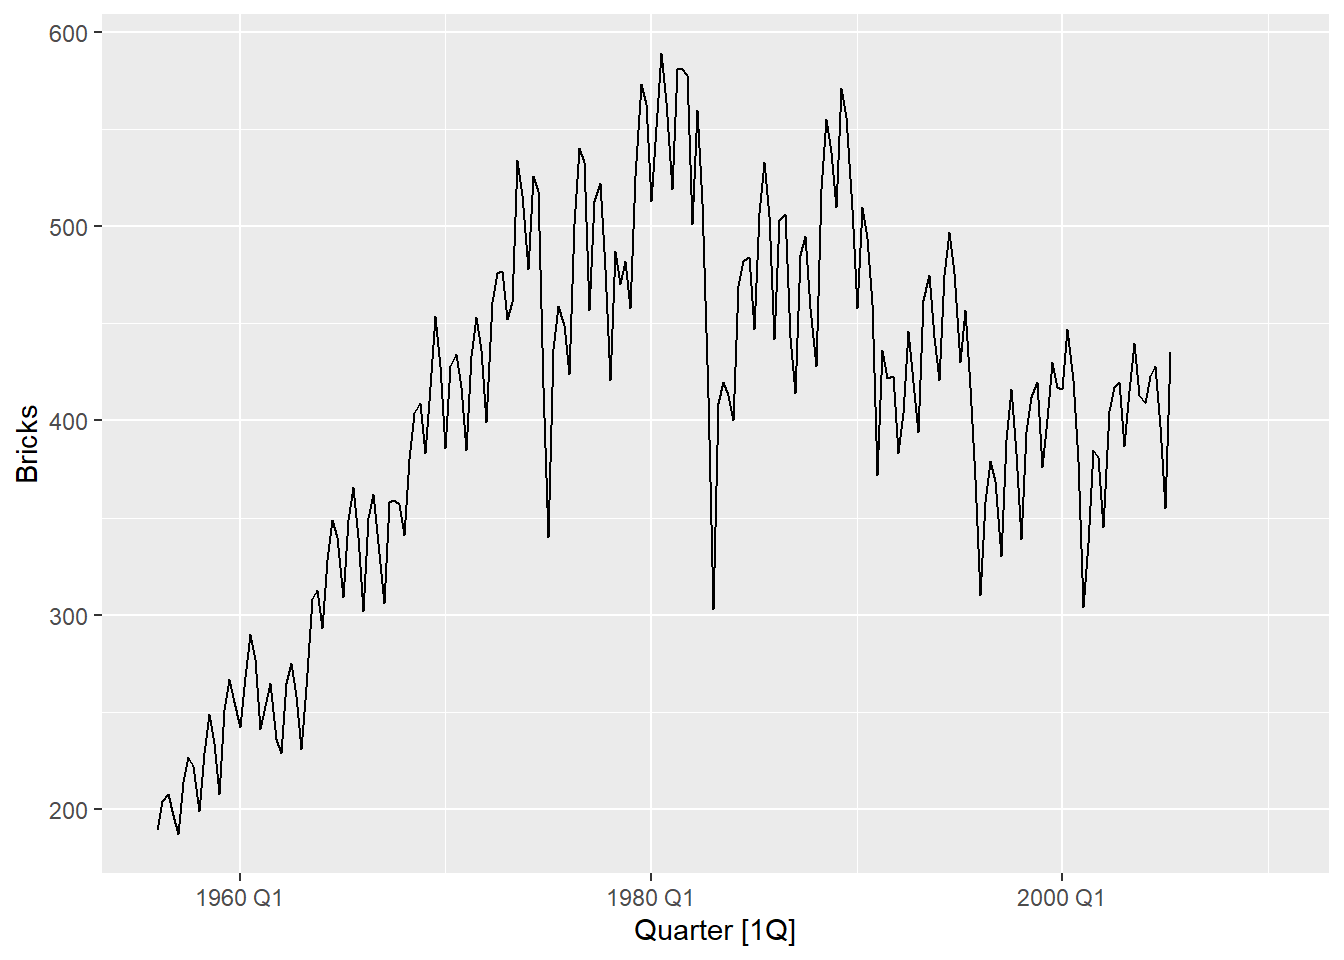
\includegraphics{Lab-9_files/figure-latex/unnamed-chunk-7-1.pdf}

\begin{enumerate}
\def\labelenumi{\arabic{enumi}.}
\setcounter{enumi}{7}
\tightlist
\item
  Is \texttt{bty\_avg} still a significant predictor of \texttt{score}?
  Has the addition of \texttt{gender} to the model changed the parameter
  estimate for \texttt{bty\_avg}?
\end{enumerate}

bty\_avg is still a significant predictor of score. The addition of
gender to the model descrease the coefficient for bty\_avg and lowered
the R-squared value as well

Note that the estimate for \texttt{gender} is now called
\texttt{gendermale}. You'll see this name change whenever you introduce
a categorical variable. The reason is that R recodes \texttt{gender}
from having the values of \texttt{male} and \texttt{female} to being an
indicator variable called \texttt{gendermale} that takes a value of
\(0\) for female professors and a value of \(1\) for male professors.
(Such variables are often referred to as ``dummy'' variables.)

As a result, for female professors, the parameter estimate is multiplied
by zero, leaving the intercept and slope form familiar from simple
regression.

\[
  \begin{aligned}
\widehat{score} &= \hat{\beta}_0 + \hat{\beta}_1 \times bty\_avg + \hat{\beta}_2 \times (0) \\
&= \hat{\beta}_0 + \hat{\beta}_1 \times bty\_avg\end{aligned}
\]

\begin{Shaded}
\begin{Highlighting}[]
\FunctionTok{ggplot}\NormalTok{(}\AttributeTok{data =}\NormalTok{ evals, }\FunctionTok{aes}\NormalTok{(}\AttributeTok{x =}\NormalTok{ bty\_avg, }\AttributeTok{y =}\NormalTok{ score, }\AttributeTok{color =}\NormalTok{ pic\_color)) }\SpecialCharTok{+} \FunctionTok{geom\_smooth}\NormalTok{(}\AttributeTok{method =} \StringTok{"lm"}\NormalTok{,}
    \AttributeTok{formula =}\NormalTok{ y }\SpecialCharTok{\textasciitilde{}}\NormalTok{ x, }\AttributeTok{se =} \ConstantTok{FALSE}\NormalTok{)}
\end{Highlighting}
\end{Shaded}

\includegraphics{Lab-9_files/figure-latex/twoLines-1.pdf}

\begin{enumerate}
\def\labelenumi{\arabic{enumi}.}
\setcounter{enumi}{8}
\tightlist
\item
  What is the equation of the line corresponding to those with color
  pictures? (\emph{Hint:} For those with color pictures, the parameter
  estimate is multiplied by 1.) For two professors who received the same
  beauty rating, which color picture tends to have the higher course
  evaluation score?
\end{enumerate}

\begin{quote}
The equation of the color line is \[
\widehat{score} = 3.47 + 0.07 bty\_avg + 0.17(0)
\]
\end{quote}

For two professors who received the same beauty rating white\&black
professors tends to score higher than color.

The decision to call the indicator variable \texttt{gendermale} instead
of \texttt{genderfemale} has no deeper meaning. R simply codes the
category that comes first alphabetically as a \(0\). (You can change the
reference level of a categorical variable, which is the level that is
coded as a 0, using the\texttt{relevel()} function. Use
\texttt{?relevel} to learn more.)

\begin{enumerate}
\def\labelenumi{\arabic{enumi}.}
\setcounter{enumi}{9}
\tightlist
\item
  Create a new model called \texttt{m\_bty\_rank} with \texttt{gender}
  removed and \texttt{rank} added in. How does R appear to handle
  categorical variables that have more than two levels? Note that the
  rank variable has three levels: \texttt{teaching},
  \texttt{tenure\ track}, \texttt{tenured}.
\end{enumerate}

\begin{Shaded}
\begin{Highlighting}[]
\NormalTok{m\_bty\_rank }\OtherTok{\textless{}{-}} \FunctionTok{lm}\NormalTok{(score }\SpecialCharTok{\textasciitilde{}}\NormalTok{ bty\_avg }\SpecialCharTok{+}\NormalTok{ rank, }\AttributeTok{data =}\NormalTok{ evals)}
\FunctionTok{summary}\NormalTok{(m\_bty\_rank)}
\end{Highlighting}
\end{Shaded}

\begin{verbatim}
## 
## Call:
## lm(formula = score ~ bty_avg + rank, data = evals)
## 
## Residuals:
##     Min      1Q  Median      3Q     Max 
## -1.8713 -0.3642  0.1489  0.4103  0.9525 
## 
## Coefficients:
##                  Estimate Std. Error t value Pr(>|t|)    
## (Intercept)       3.98155    0.09078  43.860  < 2e-16 ***
## bty_avg           0.06783    0.01655   4.098 4.92e-05 ***
## ranktenure track -0.16070    0.07395  -2.173   0.0303 *  
## ranktenured      -0.12623    0.06266  -2.014   0.0445 *  
## ---
## Signif. codes:  0 '***' 0.001 '**' 0.01 '*' 0.05 '.' 0.1 ' ' 1
## 
## Residual standard error: 0.5328 on 459 degrees of freedom
## Multiple R-squared:  0.04652,    Adjusted R-squared:  0.04029 
## F-statistic: 7.465 on 3 and 459 DF,  p-value: 6.88e-05
\end{verbatim}

The interpretation of the coefficients in multiple regression is
slightly different from that of simple regression. The estimate for
\texttt{bty\_avg} reflects how much higher a group of professors is
expected to score if they have a beauty rating that is one point higher
\emph{while holding all other variables constant}. In this case, that
translates into considering only professors of the same rank with
\texttt{bty\_avg} scores that are one point apart.

\hypertarget{the-search-for-the-best-model}{%
\subsection{The search for the best
model}\label{the-search-for-the-best-model}}

We will start with a full model that predicts professor score based on
rank, gender, ethnicity, language of the university where they got their
degree, age, proportion of students that filled out evaluations, class
size, course level, number of professors, number of credits, average
beauty rating, outfit, and picture color.

\begin{enumerate}
\def\labelenumi{\arabic{enumi}.}
\setcounter{enumi}{10}
\tightlist
\item
  Which variable would you expect to have the highest p-value in this
  model? Why? \emph{Hint:} Think about which variable would you expect
  to not have any association with the professor score.
\end{enumerate}

The variable with highest p value is cls\_prof because the number of
professors teaching would not impact model since we are taking look at
individual professor rating.

Let's run the model\ldots{}

\begin{Shaded}
\begin{Highlighting}[]
\NormalTok{m\_full }\OtherTok{\textless{}{-}} \FunctionTok{lm}\NormalTok{(score }\SpecialCharTok{\textasciitilde{}}\NormalTok{ rank }\SpecialCharTok{+}\NormalTok{ gender }\SpecialCharTok{+}\NormalTok{ ethnicity }\SpecialCharTok{+}\NormalTok{ language }\SpecialCharTok{+}\NormalTok{ age }\SpecialCharTok{+}\NormalTok{ cls\_perc\_eval }
             \SpecialCharTok{+}\NormalTok{ cls\_students }\SpecialCharTok{+}\NormalTok{ cls\_level }\SpecialCharTok{+}\NormalTok{ cls\_profs }\SpecialCharTok{+}\NormalTok{ cls\_credits }\SpecialCharTok{+}\NormalTok{ bty\_avg }
             \SpecialCharTok{+}\NormalTok{ pic\_outfit }\SpecialCharTok{+}\NormalTok{ pic\_color, }\AttributeTok{data =}\NormalTok{ evals)}
\FunctionTok{summary}\NormalTok{(m\_full)}
\end{Highlighting}
\end{Shaded}

\begin{verbatim}
## 
## Call:
## lm(formula = score ~ rank + gender + ethnicity + language + age + 
##     cls_perc_eval + cls_students + cls_level + cls_profs + cls_credits + 
##     bty_avg + pic_outfit + pic_color, data = evals)
## 
## Residuals:
##      Min       1Q   Median       3Q      Max 
## -1.77397 -0.32432  0.09067  0.35183  0.95036 
## 
## Coefficients:
##                         Estimate Std. Error t value Pr(>|t|)    
## (Intercept)            4.0952141  0.2905277  14.096  < 2e-16 ***
## ranktenure track      -0.1475932  0.0820671  -1.798  0.07278 .  
## ranktenured           -0.0973378  0.0663296  -1.467  0.14295    
## gendermale             0.2109481  0.0518230   4.071 5.54e-05 ***
## ethnicitynot minority  0.1234929  0.0786273   1.571  0.11698    
## languagenon-english   -0.2298112  0.1113754  -2.063  0.03965 *  
## age                   -0.0090072  0.0031359  -2.872  0.00427 ** 
## cls_perc_eval          0.0053272  0.0015393   3.461  0.00059 ***
## cls_students           0.0004546  0.0003774   1.205  0.22896    
## cls_levelupper         0.0605140  0.0575617   1.051  0.29369    
## cls_profssingle       -0.0146619  0.0519885  -0.282  0.77806    
## cls_creditsone credit  0.5020432  0.1159388   4.330 1.84e-05 ***
## bty_avg                0.0400333  0.0175064   2.287  0.02267 *  
## pic_outfitnot formal  -0.1126817  0.0738800  -1.525  0.12792    
## pic_colorcolor        -0.2172630  0.0715021  -3.039  0.00252 ** 
## ---
## Signif. codes:  0 '***' 0.001 '**' 0.01 '*' 0.05 '.' 0.1 ' ' 1
## 
## Residual standard error: 0.498 on 448 degrees of freedom
## Multiple R-squared:  0.1871, Adjusted R-squared:  0.1617 
## F-statistic: 7.366 on 14 and 448 DF,  p-value: 6.552e-14
\end{verbatim}

\begin{enumerate}
\def\labelenumi{\arabic{enumi}.}
\setcounter{enumi}{11}
\tightlist
\item
  Check your suspicions from the previous exercise. Include the model
  output in your response.
\end{enumerate}

\begin{Shaded}
\begin{Highlighting}[]
\NormalTok{sus\_lm }\OtherTok{\textless{}{-}} \FunctionTok{lm}\NormalTok{(score }\SpecialCharTok{\textasciitilde{}}\NormalTok{ cls\_profs, }\AttributeTok{data =}\NormalTok{ evals)}
\FunctionTok{summary}\NormalTok{(sus\_lm)}
\end{Highlighting}
\end{Shaded}

\begin{verbatim}
## 
## Call:
## lm(formula = score ~ cls_profs, data = evals)
## 
## Residuals:
##     Min      1Q  Median      3Q     Max 
## -1.8554 -0.3846  0.1154  0.4154  0.8446 
## 
## Coefficients:
##                 Estimate Std. Error t value Pr(>|t|)    
## (Intercept)      4.18464    0.03111 134.493   <2e-16 ***
## cls_profssingle -0.02923    0.05343  -0.547    0.585    
## ---
## Signif. codes:  0 '***' 0.001 '**' 0.01 '*' 0.05 '.' 0.1 ' ' 1
## 
## Residual standard error: 0.5443 on 461 degrees of freedom
## Multiple R-squared:  0.0006486,  Adjusted R-squared:  -0.001519 
## F-statistic: 0.2992 on 1 and 461 DF,  p-value: 0.5847
\end{verbatim}

We see that cls\_profs is not a significant predictor of score and very
low R squared indicates that the model is not a good fit. In addition, a
small F statistic and high p value further indicates that this variable
is not significant

\begin{enumerate}
\def\labelenumi{\arabic{enumi}.}
\setcounter{enumi}{12}
\tightlist
\item
  Interpret the coefficient associated with the ethnicity variable.
\end{enumerate}

The coefficient of ethnictiy in the model is 0.123 with p-value of
0.1169 which suggests that this varaible is nto a significable indicator
for score

\begin{enumerate}
\def\labelenumi{\arabic{enumi}.}
\setcounter{enumi}{13}
\tightlist
\item
  Drop the variable with the highest p-value and re-fit the model. Did
  the coefficients and significance of the other explanatory variables
  change? (One of the things that makes multiple regression interesting
  is that coefficient estimates depend on the other variables that are
  included in the model.) If not, what does this say about whether or
  not the dropped variable was collinear with the other explanatory
  variables?
\end{enumerate}

\begin{Shaded}
\begin{Highlighting}[]
\NormalTok{another\_lm }\OtherTok{\textless{}{-}} \FunctionTok{lm}\NormalTok{(score }\SpecialCharTok{\textasciitilde{}}\NormalTok{ rank }\SpecialCharTok{+}\NormalTok{ gender }\SpecialCharTok{+}\NormalTok{ ethnicity }\SpecialCharTok{+}\NormalTok{ language }\SpecialCharTok{+}\NormalTok{ age }\SpecialCharTok{+}\NormalTok{ cls\_perc\_eval }\SpecialCharTok{+}
\NormalTok{    cls\_students }\SpecialCharTok{+}\NormalTok{ cls\_level }\SpecialCharTok{+}\NormalTok{ cls\_credits }\SpecialCharTok{+}\NormalTok{ bty\_avg }\SpecialCharTok{+}\NormalTok{ pic\_outfit }\SpecialCharTok{+}\NormalTok{ pic\_color, }\AttributeTok{data =}\NormalTok{ evals)}
\FunctionTok{summary}\NormalTok{(another\_lm)}
\end{Highlighting}
\end{Shaded}

\begin{verbatim}
## 
## Call:
## lm(formula = score ~ rank + gender + ethnicity + language + age + 
##     cls_perc_eval + cls_students + cls_level + cls_credits + 
##     bty_avg + pic_outfit + pic_color, data = evals)
## 
## Residuals:
##     Min      1Q  Median      3Q     Max 
## -1.7836 -0.3257  0.0859  0.3513  0.9551 
## 
## Coefficients:
##                         Estimate Std. Error t value Pr(>|t|)    
## (Intercept)            4.0872523  0.2888562  14.150  < 2e-16 ***
## ranktenure track      -0.1476746  0.0819824  -1.801 0.072327 .  
## ranktenured           -0.0973829  0.0662614  -1.470 0.142349    
## gendermale             0.2101231  0.0516873   4.065 5.66e-05 ***
## ethnicitynot minority  0.1274458  0.0772887   1.649 0.099856 .  
## languagenon-english   -0.2282894  0.1111305  -2.054 0.040530 *  
## age                   -0.0089992  0.0031326  -2.873 0.004262 ** 
## cls_perc_eval          0.0052888  0.0015317   3.453 0.000607 ***
## cls_students           0.0004687  0.0003737   1.254 0.210384    
## cls_levelupper         0.0606374  0.0575010   1.055 0.292200    
## cls_creditsone credit  0.5061196  0.1149163   4.404 1.33e-05 ***
## bty_avg                0.0398629  0.0174780   2.281 0.023032 *  
## pic_outfitnot formal  -0.1083227  0.0721711  -1.501 0.134080    
## pic_colorcolor        -0.2190527  0.0711469  -3.079 0.002205 ** 
## ---
## Signif. codes:  0 '***' 0.001 '**' 0.01 '*' 0.05 '.' 0.1 ' ' 1
## 
## Residual standard error: 0.4974 on 449 degrees of freedom
## Multiple R-squared:  0.187,  Adjusted R-squared:  0.1634 
## F-statistic: 7.943 on 13 and 449 DF,  p-value: 2.336e-14
\end{verbatim}

\begin{enumerate}
\def\labelenumi{\arabic{enumi}.}
\setcounter{enumi}{14}
\tightlist
\item
  Using backward-selection and p-value as the selection criterion,
  determine the best model. You do not need to show all steps in your
  answer, just the output for the final model. Also, write out the
  linear model for predicting score based on the final model you settle
  on.
\end{enumerate}

\begin{Shaded}
\begin{Highlighting}[]
\NormalTok{best\_lm }\OtherTok{\textless{}{-}} \FunctionTok{lm}\NormalTok{(score }\SpecialCharTok{\textasciitilde{}}\NormalTok{ gender }\SpecialCharTok{+}\NormalTok{ language }\SpecialCharTok{+}\NormalTok{ age }\SpecialCharTok{+}\NormalTok{ cls\_perc\_eval }\SpecialCharTok{+}\NormalTok{ cls\_credits }\SpecialCharTok{+}\NormalTok{ bty\_avg }\SpecialCharTok{+}
\NormalTok{    pic\_color, }\AttributeTok{data =}\NormalTok{ evals)}
\FunctionTok{summary}\NormalTok{(best\_lm)}
\end{Highlighting}
\end{Shaded}

\begin{verbatim}
## 
## Call:
## lm(formula = score ~ gender + language + age + cls_perc_eval + 
##     cls_credits + bty_avg + pic_color, data = evals)
## 
## Residuals:
##      Min       1Q   Median       3Q      Max 
## -1.81919 -0.32035  0.09272  0.38526  0.88213 
## 
## Coefficients:
##                        Estimate Std. Error t value Pr(>|t|)    
## (Intercept)            3.967255   0.215824  18.382  < 2e-16 ***
## gendermale             0.221457   0.049937   4.435 1.16e-05 ***
## languagenon-english   -0.281933   0.098341  -2.867  0.00434 ** 
## age                   -0.005877   0.002622  -2.241  0.02551 *  
## cls_perc_eval          0.004295   0.001432   2.999  0.00286 ** 
## cls_creditsone credit  0.444392   0.100910   4.404 1.33e-05 ***
## bty_avg                0.048679   0.016974   2.868  0.00432 ** 
## pic_colorcolor        -0.216556   0.066625  -3.250  0.00124 ** 
## ---
## Signif. codes:  0 '***' 0.001 '**' 0.01 '*' 0.05 '.' 0.1 ' ' 1
## 
## Residual standard error: 0.5014 on 455 degrees of freedom
## Multiple R-squared:  0.1631, Adjusted R-squared:  0.1502 
## F-statistic: 12.67 on 7 and 455 DF,  p-value: 6.996e-15
\end{verbatim}

\begin{enumerate}
\def\labelenumi{\arabic{enumi}.}
\setcounter{enumi}{15}
\tightlist
\item
  Verify that the conditions for this model are reasonable using
  diagnostic plots.
\end{enumerate}

\begin{Shaded}
\begin{Highlighting}[]
\FunctionTok{qqnorm}\NormalTok{(best\_lm}\SpecialCharTok{$}\NormalTok{residuals)}
\FunctionTok{qqline}\NormalTok{(best\_lm}\SpecialCharTok{$}\NormalTok{residuals)}
\end{Highlighting}
\end{Shaded}

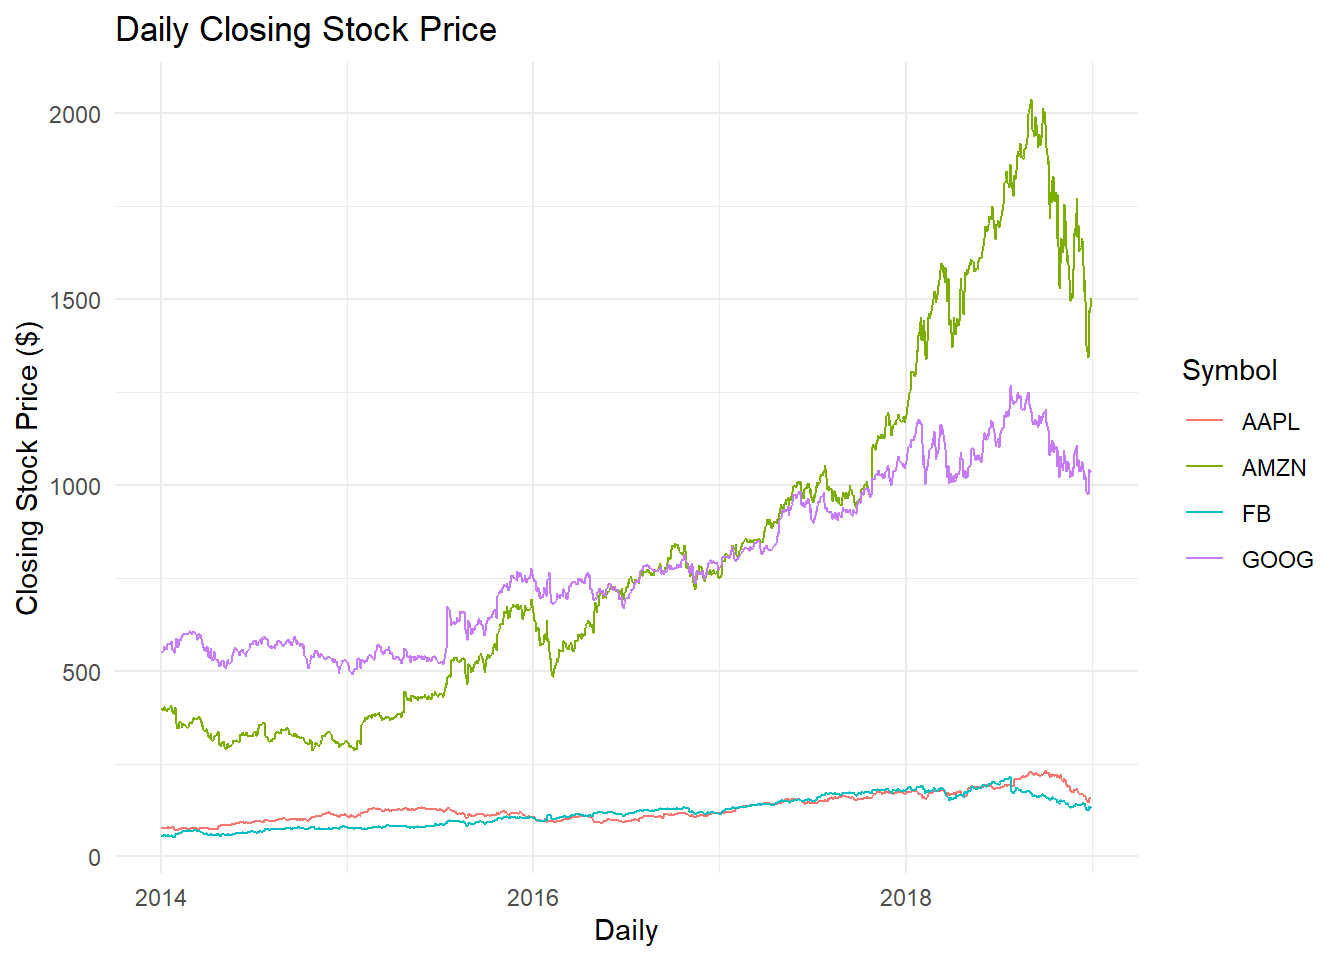
\includegraphics{Lab-9_files/figure-latex/unnamed-chunk-12-1.pdf}

\begin{enumerate}
\def\labelenumi{\arabic{enumi}.}
\setcounter{enumi}{16}
\tightlist
\item
  The original paper describes how these data were gathered by taking a
  sample of professors from the University of Texas at Austin and
  including all courses that they have taught. Considering that each row
  represents a course, could this new information have an impact on any
  of the conditions of linear regression?
\end{enumerate}

It might have an impact on the regression becuase some courses will be
taught by the same professors which may introduce bias in the analysis.

\begin{enumerate}
\def\labelenumi{\arabic{enumi}.}
\setcounter{enumi}{17}
\tightlist
\item
  Based on your final model, describe the characteristics of a professor
  and course at University of Texas at Austin that would be associated
  with a high evaluation score.
\end{enumerate}

The most significant characteritics of a professor to receive a high
evaluation score are if they are black\&white english speaking male
teaching a multi credit course

\begin{enumerate}
\def\labelenumi{\arabic{enumi}.}
\setcounter{enumi}{18}
\tightlist
\item
  Would you be comfortable generalizing your conclusions to apply to
  professors generally (at any university)? Why or why not?
\end{enumerate}

It would be not be right to generalize conculsion infered from a sample
from one universtiy and apply it to any universities without first
taking samples from every other university. So no, I would not be
comfortable generalizing this conclusions.

\begin{center}\rule{0.5\linewidth}{0.5pt}\end{center}

\end{document}
